\chapter{APIs del Sistema}
\label{anx:apis}

En este anexo incluimos la definición de todas las APIs de los microservicios del sistema. Esto incluye los \foreign{english}{endponts} HTTP, las notificaciones y las peticiones asíncronas. Se listan en orden de intervención en el proceso de adaptación.

\section{Bucle de adaptación}

\subsection{Monitorización}

\subsubsection{Peticiones síncronas}

Su especificación OpenAPI puede encontrarse \href{https://github.com/Starkie/TFM-DistributedAutoadaptiveSystems/blob/3300a2e54ce0fe82701d53c3d3cb6cbcd64141be/src/AutoAdaptativeSystem/AdaptionLoop/Monitoring/Monitoring.Service-OpenAPISpec.json}{aquí}.

\begin{figure}[h!]
  \hspace{-0.25cm}
  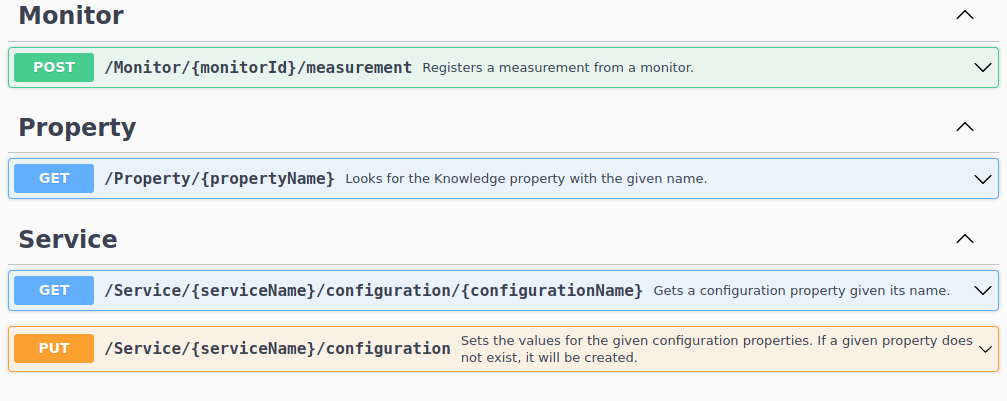
\includegraphics[scale=0.45]{anx_apis/images/apis-monitoring}
  \caption{\foreign{english}{Endponts} HTTP que expone el servicio de monitorización.}
\end{figure}

\subsection{Conocimiento}

\subsubsection{Peticiones síncronas}

Su especificación OpenAPI puede encontrarse \href{https://github.com/Starkie/TFM-DistributedAutoadaptiveSystems/blob/3300a2e54ce0fe82701d53c3d3cb6cbcd64141be/src/AutoAdaptativeSystem/AdaptionLoop/Knowledge/Knowledge.Service-OpenAPISpec.json}{aquí}.

\begin{figure}[h!]
  \hspace{-0.25cm}
  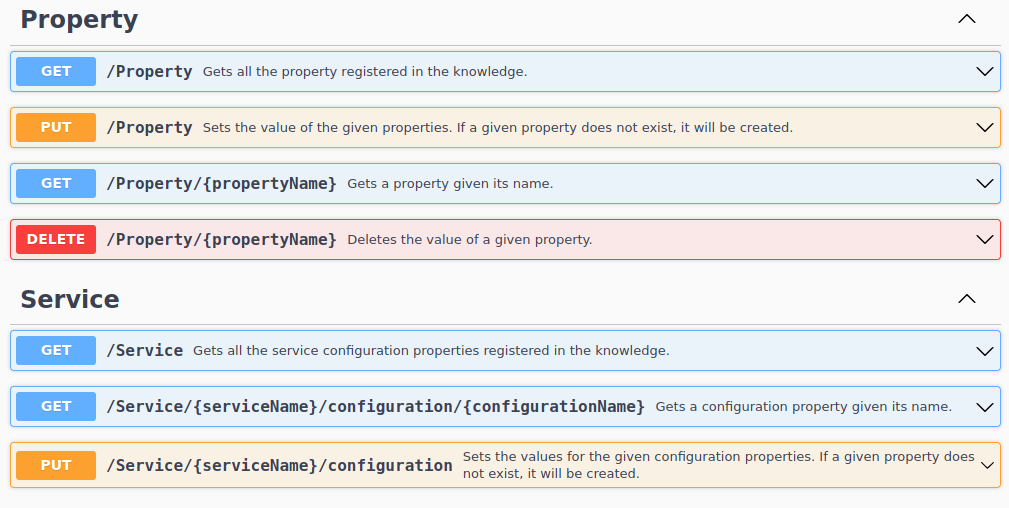
\includegraphics[scale=0.45]{anx_apis/images/apis-knowledge}
  \caption{\foreign{english}{Endponts} HTTP que expone el servicio de conocimiento.}
\end{figure}

\pagebreak

\subsubsection{Notificaciones}

\newsavebox\configurationchangedeventbox
\begin{lrbox}{\configurationchangedeventbox}
  \begin{minipage}[t]{2in}
    \begin{verbatim}
{
  "ServiceName":"Climatisation.AirConditioner.Service",
  "ConfigurationName":"TargetTemperature",
}
        \end{verbatim}
  \end{minipage}
\end{lrbox}

\begin{longtable}{|m{2.3cm}|p{3cm}|p{2.6cm}|b{1.5cm}|b{1cm}|}
  \hline

  \textbf{Evento} & \multicolumn{4}{|b{0.7\linewidth}|}{\emph{PropertyChangedIntegrationEvent }} \\
  \hline

  \textbf{\emph{Exchange}} & \multicolumn{4}{|b{0.7\linewidth}|}{\emph{AdaptionLoop.Knowledge}} \\
  \hline

  \textbf{Tema} & \multicolumn{4}{|b{0.7\linewidth}|}{\emph{PropertyChangedIntegrationEvent}} \\
  \hline

  \textbf{Descripción} & \multicolumn{4}{|b{0.6\linewidth}|}{Evento de integración que notifica sobre el cambio de una propiedad adaptación.} \\
  \hline

  \textbf{Propiedades}
        & \emph{propertyName} & \multicolumn{3}{|b{0.6\linewidth}|}{Nombre de la propiedad que ha cambiado.} \\
  \hline

  \textbf{Ejemplo} & \multicolumn{4}{|b{0.7\linewidth}|}{Evento que notifica del cambio de la propiedad \emph{Temperature}:\linebreak
  \usebox\propertychangedeventbox} \\

  \hline
  \hline

  \textbf{Evento} & \multicolumn{4}{|b{0.7\linewidth}|}{\emph{ConfigurationChangedIntegrationEvent}} \\
  \hline

  \textbf{\emph{Exchange}} & \multicolumn{4}{|b{0.7\linewidth}|}{\emph{AdaptionLoop.Knowledge}}  \\
  \hline

  \textbf{Tema} & \multicolumn{4}{|b{0.7\linewidth}|}{\emph{ConfigurationChangedIntegrationEvent}} \\
  \hline

  \textbf{Descripción} & \multicolumn{4}{|b{0.6\linewidth}|}{Evento de integración que notifica sobre el cambio de una clave de configuración.} \\
  \hline

  \textbf{Propiedades}
        & \emph{serviceName} & \multicolumn{3}{|b{0.6\linewidth}|}{Nombre del servicio al que pertenece.} \\

        \cline{2-5}

        & \emph{configurationName} & \multicolumn{3}{|b{0.6\linewidth}|}{Nombre de la clave de configuración que ha cambiado.} \\
  \hline

  \textbf{Ejemplo} & \multicolumn{4}{|b{0.7\linewidth}|}{Evento que notifica del cambio de la propiedad de configuración \emph{TargetTemperature}:\linebreak
  \usebox\configurationchangedeventbox} \\

  \hline

  \caption{Especificación de las notificaciones que publica el servicio de conocimiento.}
\end{longtable}


\subsection{Análisis}

\subsubsection{Peticiones síncronas}

Su especificación OpenAPI puede encontrarse \href{https://github.com/Starkie/TFM-DistributedAutoadaptiveSystems/blob/3300a2e54ce0fe82701d53c3d3cb6cbcd64141be/src/AutoAdaptativeSystem/AdaptionLoop/Analysis/Analysis.Service-OpenAPISpec.json}{aquí}.

\begin{figure}[h!]
  \hspace{-0.25cm}
  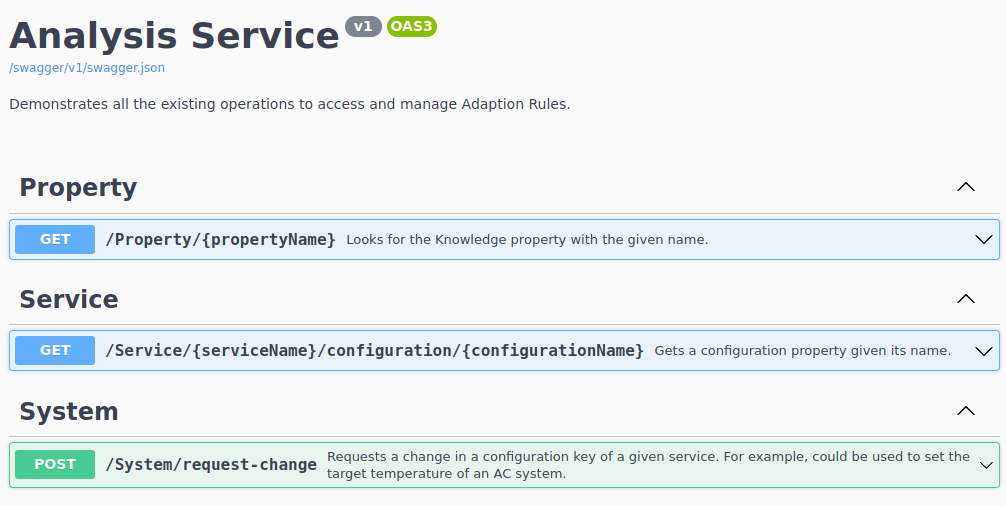
\includegraphics[scale=0.45]{anx_apis/images/apis-analysis}
  \caption{\foreign{english}{Endponts} HTTP que expone el servicio de análisis.}
\end{figure}

\subsubsection{Notificaciones}

\begin{longtable}{|m{2.3cm}|p{3cm}|p{2.6cm}|b{1.5cm}|b{1cm}|}
  \hline

  \textbf{Evento} & \multicolumn{4}{|b{0.7\linewidth}|}{\emph{PropertyChangedIntegrationEvent }} \\
  \hline

  \textbf{\emph{Exchange}} & \multicolumn{4}{|b{0.7\linewidth}|}{\emph{AdaptionLoop.Analysis}} \\
  \hline

  \textbf{Tema} & \multicolumn{4}{|b{0.7\linewidth}|}{Nombre de la propiedad. Ej: \emph{Temperature}} \\
  \hline

  \textbf{Descripción} & \multicolumn{4}{|b{0.6\linewidth}|}{Evento de integración que notifica sobre el cambio de una propiedad adaptación.} \\
  \hline

  \textbf{Propiedades}
        & \emph{propertyName} & \multicolumn{3}{|b{0.6\linewidth}|}{Nombre de la propiedad que ha cambiado.} \\
  \hline

  \textbf{Ejemplo} & \multicolumn{4}{|b{0.7\linewidth}|}{Evento que notifica del cambio de la propiedad \emph{Temperature}:\linebreak
  \usebox\propertychangedeventbox} \\

  \hline
  \hline

  \textbf{Evento} & \multicolumn{4}{|b{0.7\linewidth}|}{\emph{ConfigurationChangedIntegrationEvent}} \\
  \hline

  \textbf{\emph{Exchange}} & \multicolumn{4}{|b{0.7\linewidth}|}{\emph{AdaptionLoop.Analysis}}  \\
  \hline

  \textbf{Tema} & \multicolumn{4}{|b{0.7\linewidth}|}{Nombre del servicio y la propiedad. Ej: \emph{Climatisation.AirConditioner.TargetTemperature}} \\
  \hline

  \textbf{Descripción} & \multicolumn{4}{|b{0.6\linewidth}|}{Evento de integración que notifica sobre el cambio de una clave de configuración.} \\
  \hline

  \textbf{Propiedades}
        & \emph{serviceName} & \multicolumn{3}{|b{0.6\linewidth}|}{Nombre del servicio al que pertenece.} \\

        \cline{2-5}

        & \emph{configurationName} & \multicolumn{3}{|b{0.6\linewidth}|}{Nombre de la clave de configuración que ha cambiado.} \\
  \hline

  \textbf{Ejemplo} & \multicolumn{4}{|b{0.7\linewidth}|}{Evento que notifica del cambio de la propiedad de configuración \emph{TargetTemperature}:\linebreak
  \usebox\configurationchangedeventbox} \\

  \hline

  \caption{Especificación de las notificaciones que publica el servicio de análisis.}
\end{longtable}

\subsection{Planificador}

\subsubsection{Peticiones asíncronas}

\begin{longtable}{|m{2cm}|m{2.3cm}|m{10cm}|b{0.85cm}|b{2.75cm}|}
  \hline

  \textbf{Peticion} & \multicolumn{4}{|b{0.7\linewidth}|}{\emph{SystemConfigurationChangeRequest}} \\
  \hline

  \textbf{\emph{Cola}} & \multicolumn{4}{|b{0.7\linewidth}|}{\emph{AdaptionLoop.Planification.Requests}} \\
  \hline

  \textbf{Descripción} & \multicolumn{4}{|b{0.82\linewidth}|}{Petición que representa una propuesta de cambio de la configuración del sistema.} \\
  \hline

  \textbf{Propiedades}
    & \emph{Timestamp} & \multicolumn{3}{|m{0.67\linewidth}|}{Fecha y hora de la petición de cambio.} \\
    \cline{2-5}
    & \emph{Symptoms} & \multicolumn{3}{|m{0.67\linewidth}|}{Colección de síntomas que la han desencadenado.} \\
    \cline{2-5}
    & \emph{Configuration Requests} & \multicolumn{3}{|m{0.67\linewidth}|}{Colección peticiones de configuración de la propuesta de cambio. Cada una de estas está compuesta por:
    \begin{itemize}[noitemsep]
      \item \textbf{\emph{ServiceName}}: Identificador del servicio cuya configuración queremos cambiar.
      \item \textbf{\emph{IsDeployed}}: Indica si el servicio debe estar desplegado o no en la siguiente configuración.
      \item \textbf{\emph{Bindings}}: Colección de conexiones que indican a qué otros servicios debe estar conectado (o no) en la siguiente configuración.
      \item \textbf{\emph{ConfigurationProperties}}: Colección de pares clave-valor que representan valores de su configuración que queremos actualizar.
    \end{itemize}} \\
  \hline

  \textbf{Ejemplo} & \multicolumn{4}{|b{0.82\linewidth}|}{Solicitud de cambio del modo de un aire acondicionado a modo calefacción (\emph{heating}). Los síntomas indican que fue desencadenada porque la temperatura era menor que un umbral determinado:\linebreak
  \usebox\systemconfigurationchangerequestbox} \\

  \hline

  \caption{Especificación de la petición asíncrona que expone el planificador.}
\end{longtable}

\subsection{Ejecutor}

\subsubsection{Peticiones asíncronas}

\newsavebox\executechangeplanrequestbox
\begin{lrbox}{\executechangeplanrequestbox}
  \begin{minipage}[t]{2in}
    \begin{verbatim}
{
  "Timestamp": "2022-06-19T16:38:30.6092751Z",
  "Symptoms":[
    {
      "Name": "temperature-lesser-than-cold-threshold",
      "Value": "true"
    }
  ],
  "ChangePlan":  [
    {
      "ServiceName": "Climatisation.AirConditioner.Service",
      "Type": "SetParameter",
      "PropertyName": "Mode",
      "PropertyValue": "Heating"
    }
  ]
}
        \end{verbatim}
  \end{minipage}
\end{lrbox}

\begin{longtable}{|m{2cm}|m{2.3cm}|m{10cm}|b{0.85cm}|b{2.75cm}|}
  \hline

  \textbf{Peticion} & \multicolumn{4}{|b{0.7\linewidth}|}{\emph{ExecuteChangePlanRequest}} \\
  \hline

  \textbf{\emph{Cola}} & \multicolumn{4}{|b{0.7\linewidth}|}{\emph{AdaptionLoop.Execution.Requests}} \\
  \hline

  \textbf{Descripción} & \multicolumn{4}{|b{0.82\linewidth}|}{Petición para ejecutar el plan de cambio creado por el planificador.} \\
  \hline

  \textbf{Propiedades}
    & \emph{Timestamp} & \multicolumn{3}{|m{0.67\linewidth}|}{Fecha y hora en la que se generó el plan de cambio.} \\
    \cline{2-5}
    & \emph{Symptoms} & \multicolumn{3}{|m{0.67\linewidth}|}{Colección de síntomas que lo han desencadenado.} \\
    \cline{2-5}
    & \emph{ChangePlan} & \multicolumn{3}{|m{0.67\linewidth}|}{Colección de acciones de adaptación que deben ejecutarse para completar la adaptación.
    Dependiendo del tipo de acción, tendrá una estructura similar a:
    \begin{itemize}
      \item \textbf{\emph{ServiceName}}: Identificador del servicio afectado.
      \item \textbf{\emph{Type}}: Indica el tipo de acción de adaptación. Puede ser: \emph{Deploy}, \emph{Undeploy}, \emph{SetParameter}, \emph{Bind}, \emph{Unbind}.
      \item \textbf{\emph{TargetService}}: (\emph{BindingAction}) Servicio con el que establecer una conexión.
      \item \textbf{\emph{PropertyName}}: (\emph{SetParameterAction}) Nombre de la propiedad a actualizar.
      \item \textbf{\emph{PropertyValue}}: (\emph{SetParameterAction}) Valor a asignar a la propiedad.
    \end{itemize}} \\
  \hline

  \textbf{Ejemplo} & \multicolumn{4}{|b{0.82\linewidth}|}{Petición de ejecución de plan de cambio que contiene una acción de adaptación. Esta cambia el modo de un aire acondicionado a modo calefacción (\emph{heating}). Los síntomas indican que fue desencadenada porque la temperatura era menor que un umbral determinado:\linebreak
  \usebox\executechangeplanrequestbox} \\

  \hline

  \caption{Especificación de la petición asíncrona que expone el ejecutor.}
\end{longtable}

\pagebreak

\subsubsection{Notificaciones}

\newsavebox\executenotificationbox
\begin{lrbox}{\executenotificationbox}
  \begin{minipage}[t]{2in}
    \begin{verbatim}
{
  "ServiceName": "Climatisation.AirConditioner.Service",
  "Timestamp": "2022-06-19T16:38:30.6092751Z",
  "Symptoms":[
    {
      "Name": "temperature-lesser-than-cold-threshold",
      "Value": "true"
    }
  ],
  "Actions":  [
    {
      "ServiceName": "Climatisation.AirConditioner.Service",
      "Type": "SetParameter",
      "PropertyName": "Mode",
      "PropertyValue": "Heating"
    }
  ]
}
        \end{verbatim}
  \end{minipage}
\end{lrbox}

\begin{longtable}{|m{2.3cm}|p{3cm}|p{2.6cm}|b{1.5cm}|b{1cm}|}
  \hline

  \textbf{Evento} & \multicolumn{4}{|b{0.7\linewidth}|}{\emph{ExecutionRequestedIntegrationEvent}} \\
  \hline

  \textbf{\emph{Exchange}} & \multicolumn{4}{|b{0.7\linewidth}|}{\emph{AdaptionLoop.Execute}}  \\
  \hline

  \textbf{Tema} & \multicolumn{4}{|b{0.7\linewidth}|}{Nombre del servicio afectado. Ej: \emph{Climatisation.AirConditioner}} \\
  \hline

  \textbf{Descripción} & \multicolumn{4}{|b{0.6\linewidth}|}{Evento de integración que notifica sobre la solicitud de ejecución de acciones de adaptación para un servicio determinado. Se publica como notificación porque no sabemos cuantos ejecutores tendrá un determinado servicio.} \\
  \hline

  \textbf{Propiedades}
        & \emph{ServiceName} & \multicolumn{3}{|b{0.6\linewidth}|}{Nombre del servicio afectado.} \\

        \cline{2-5}

        & \emph{Timestamp} & \multicolumn{3}{|b{0.6\linewidth}|}{Fecha y hora en la que se solicitó la ejecución.} \\

        \cline{2-5}

        & \emph{Symptoms} & \multicolumn{3}{|b{0.6\linewidth}|}{Conjunto de síntomas que han desencadenado la adaptación.} \\

        \cline{2-5}

        & \emph{Actions} & \multicolumn{3}{|b{0.6\linewidth}|}{Conjunto de acciones de adaptación a ejecutar.} \\

        \cline{2-5}

  \hline

  \textbf{Ejemplo} & \multicolumn{4}{|b{0.7\linewidth}|}{Evento que notifica de la solicitud de ejecución de una acción de adaptación sobre el servicio \emph{Climatisation.AirConditioner}. Esta solicita que se cambie el parámetro \emph{Mode} a \emph{Heating}:\linebreak
  \usebox\executenotificationbox} \\

  \hline

  \caption{Especificación de las notificaciones que publica el servicio ejecución.}
\end{longtable}

\section{Sistema de climatización}

\subsection{Recurso manejado: Aire acondicionado}

\subsubsection{Peticiones síncronas}

Su especificación OpenAPI puede encontrarse \href{https://github.com/Starkie/TFM-DistributedAutoadaptiveSystems/blob/3300a2e54ce0fe82701d53c3d3cb6cbcd64141be/src/AutoAdaptativeSystem/Climatisation/AirConditioner/Service/Climatisation.AirConditioner.Service-OpenAPISpec.json}{aquí}.

\begin{figure}[h!]
  \hspace{-0.25cm}
  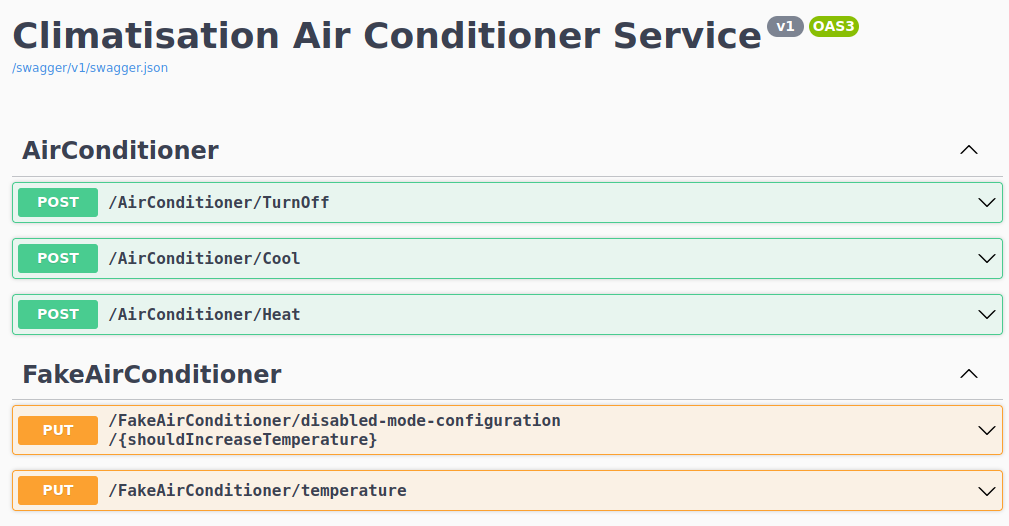
\includegraphics[scale=0.45]{anx_apis/images/apis-airconditioner}
  \caption{\foreign{english}{Endponts} HTTP que expone el recurso manejado: el aire acondicionado.}
  \label{fig:apis-eps-aireacondicionado}
\end{figure}

\subsection{Monitor}

\subsubsection{Peticiones síncronas}

Su especificación OpenAPI puede encontrarse \href{https://github.com/Starkie/TFM-DistributedAutoadaptiveSystems/blob/3300a2e54ce0fe82701d53c3d3cb6cbcd64141be/src/AutoAdaptativeSystem/Climatisation/Monitor/Climatisation.Monitor.Service-OpenAPISpec.json}{aquí}.

\begin{figure}[h!]
  \hspace{-0.25cm}
  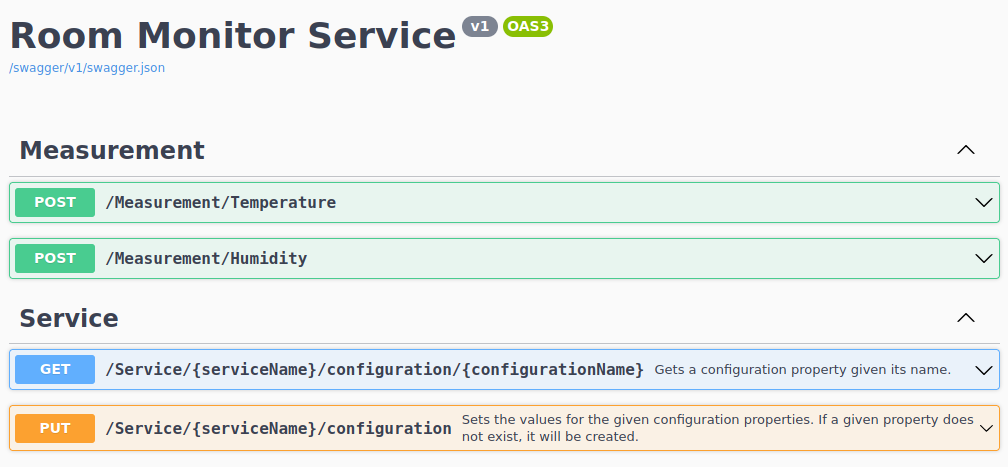
\includegraphics[scale=0.45]{anx_apis/images/apis-room-monitor}
  \caption{\foreign{english}{Endponts} HTTP que expone el servicio del monitor del sistema de climatización.}
\end{figure}
